\ifx\wholebook\relax\else
\input{../Common.tex}
\input{../macroes.tex}
\begin{document}
\fi
\chapter{Methods: Named Message Sequences}\label{ch:turtleTeaching}\label{ch:abstraction}\label{cha:enseigner}

%\begin{chapterfigure}
%
\includegraphics[width=0.9\linewidth]{carosName}
%\end{chapterfigure}

%\begin{figure}
%\center{\includegraphics{microBrowserInWorking}}
%\caption{ .\label{fig:microBrowserInWorking}}
%\end{figure}


Up to now, you used scripts: you created a robot and sent a sequence of messages to it. Using scripts is a straightforward approach, but it has some severe limitations. One of the major limitations is that a script cannot be called by another script. This is a real problem because a script cannot be reused by other scripts, you have to rewrite it again and again. 

Wouldn't it be nice if one could define a kind of script whose sequence of messages could be sent to any robot? Well, this is actually possible, and such a sequence of messages is called a \emph{method}\footnote{In the context of this book we will not go into the full power of methods, as it involves object-oriented programming.}. A \emph{method} is a named script. This name can be used in a script or even in another method.  In fact, there is nothing really new here: All the robot messages you have used so far are methods that you used with any robot!
 
 In this chapter, you shall learn how to define methods. You already know most of what you need to write the code of the methods. However a method must be defined using  a special editor called \index{code browser} \index{browser} a code browser. We start by comparing a script and a method. Then we will define a method, and finally step back and really look in detail at what we did.


\section{Scripts versus Methods}
Let's look at one of the scripts you have already written, for example script~\ref{src:againSquare} that created a robot and asked it to draw a square 100 pixels wide. 

\begin{scriptwithtitle}{A simple square}\label{src:againSquare}
| \caro |
\caro := \Turtle new.
4 timesRepeat: 
         [ \caro turnLeft: 90.
         \caro go: 100 ]
\end{scriptwithtitle}

The problem with this script is that each time you need to draw a square
you need to \emph{copy} the 3 last lines of \scriptref{src:againSquare}.  
Also if you want another robot (for example \daly) to draw the square, you must 
change the name \caro to \daly everywhere. This is illustrated by \scriptref{src:againSquare2}.

\begin{scriptwithtitle}{Two simple squares}\label{src:againSquare2}
| \caro \daly |
\caro := \Turtle new.
\daly := \Turtle new.
\daly jump: 200.
\daly color: Color red.
\textbf{
4 timesRepeat: 
         [ \caro turnLeft: 90.
         \caro go: 100 ].
4 timesRepeat: 
         [ \daly turnLeft: 90.
         \daly go: 100 ].}
\end{scriptwithtitle}

For all these reasons, working with scripts is not easy. In fact, I'm quite convinced that the following two statements reflect your personal experience with scripts.

\begin{itemize}
\item Writing long scripts is a painful task.
\item Repeating long scripts is boring and error prone. 
\item When copying complex scripts, the likelihood of making a
programming\footnote{As opposed to a syntax error, which would be
caught quickly by the computer. \emph{Programming} errors, on the
contrary, are quite difficult to catch.}  error, such as omitting a
line, is high.
\end{itemize}

Instead, we would like to \emph{define a sequence of messages once and for all;} a sequence of messages, to give the sequence a \emph{name}; and then to be able to \emph{send it as a single message to any robot} --- just like the predefined robot messages such as \go, \north, \jump... 
         
         
With this approach we could define a new \emph{method} \ct{square}, and 
then write \scriptref{src:againSquareMethod} --- but don't execute it 
yet, because the method \ct{square} has not yet been defined.  But you can see that you do not have to duplicate and adapt the sequence of messages defining a square anymore. You can just use it twice.

I hope you are now convinced that defining the method is worth the effort. 
   
\begin{scriptwithtitle}{Using the method \ct{square}}\label{src:againSquareMethod}
| \caro \daly | 
\caro := \Turtle new.  
\daly := \Turtle new.  
\daly go: 200.  
\daly color: Color red.
\textbf{\caro square.
\daly square}
\end{scriptwithtitle}


%%%%%%%%%%%%%%%%%%%%%%%%%%%%%%%%%%%%%%%%%%%%

\section{How Do We Define a Method?}
In this section we give a cookbook recipe for creating a method. In \sq you can define methods on any object but in this book you will only define methods for robots. Therefore to help you I developed a specialized code browser named Class Bot Browser just for defining methods for your robots. There is a Class Bot Browser in the working flap, or you can always create one by dragging its thumbnail from the dark blue flap or via the menu \button{open...}.

Using a Class Bot Browser to define a method requires you to (1) choose or create a method category, that is a kind of method folder (Section~\ref{sec:createCategory}), (2) type the method and (3) then compile it (see Section~\ref{sec:definingmethod}). 

Let's detail the different parts of a Class Bot Browser.

\subsection{A Class Bot Browser}

Defining methods requires a new tool: the editor shown in Figure~\ref{fig:methodEditor}. This browser is actually a simplified version of the browser used by \st programmers. 

\begin{figure}
\centerline{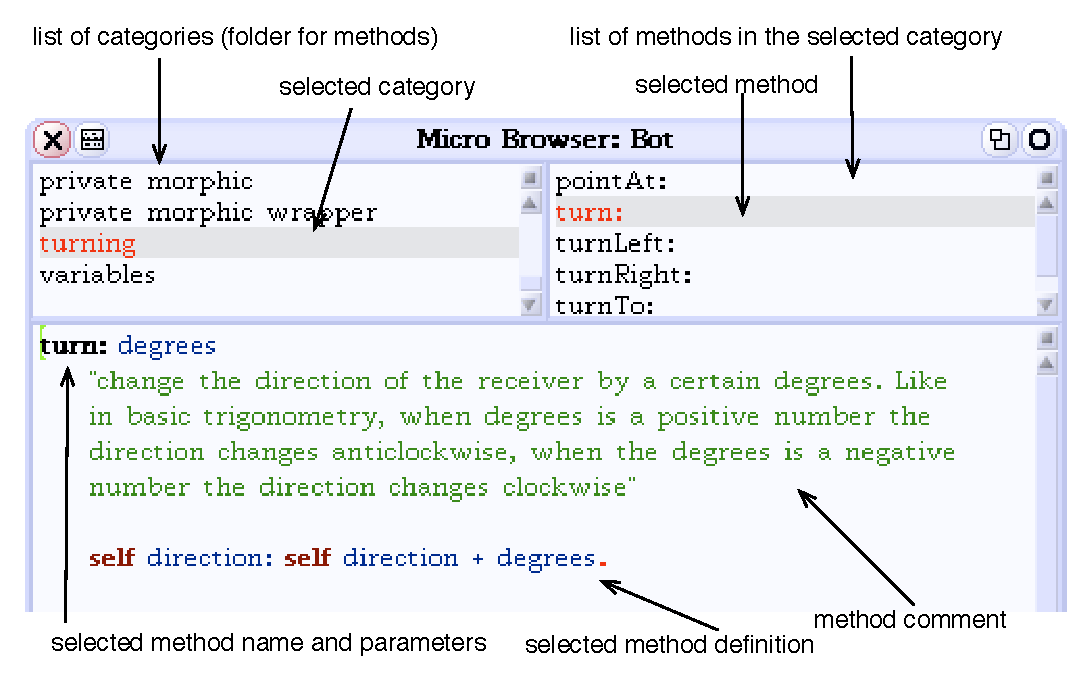
\includegraphics[width=10cm]{tbOneAnnotated}} 
\caption{A Class Bot Browser showing the definition (in the bottom pane) of the 
method \ct{turn:} (selected in the upper right pane) belonging to the category \emph{turning} (selected in the upper left pane).\label{fig:methodEditor}}
\end{figure}

The browser consists of 3 parts or panes:
\begin{description}
\item[Categories.] The upper left part is the \emph{category list}.
It shows the method categories. Method categories are just names
that group methods together so that we can find information
faster. In Figure~\ref{fig:methodEditor}, the category 'turning'
is selected; it groups all the operations having to do with robot direction changes. 
Other categories that group other robot methods are also listed.

\item[Methods.] The upper right part is the \emph{method list}.
It shows the method names of the methods  in the selected category. In Figure~\ref{fig:methodEditor}, five  methods are listed: \ct{pointAt:}, \ct{turn:}, \turnLeft, \turnRight, and \ct{turnTo:}. The method named \ct{turn:} is currently selected.

\item[Method Definition.] The bottom part is the \emph{code display and code editor}. It shows the definition of the method whose name is selected. This is also where you can type the code of a new method.

\end{description}


\subsection{Creating a New Method Category}\label{sec:createCategory} 
Methods are grouped by categories. A category is simply defined by a name. To start defining a method, you either define a new category for it, or select an existing category for your method. Let's create a new category named \ct{regular polygons}.

\begin{figure}[h]
\centerline{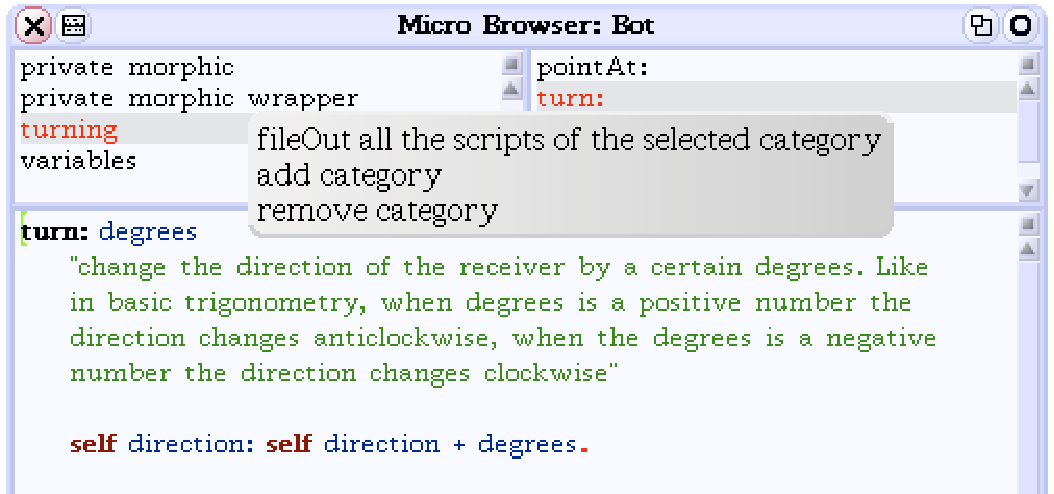
\includegraphics[width=8cm]{tbTwo}} 
\caption{To create a method category, open the category menu and select 'add category'.\label{fig:categoryMenu}}
\end{figure}
\begin{figure}\label{fig:categoryPrompt}
\centerline{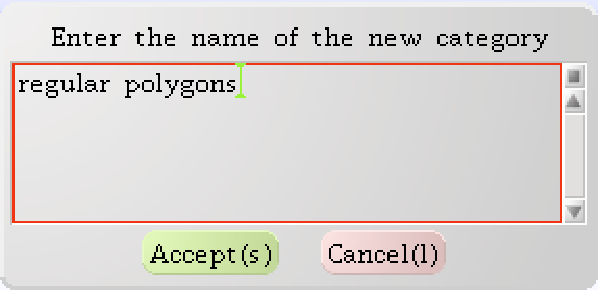
\includegraphics[width=6cm]{tbThree}}
 \caption{Entering the new category name.}
\end{figure}

\begin{enumerate}

\item Click with the right mouse button on the category list.
A menu like the one in Figure~\ref{fig:categoryMenu} will show up.

\item Select the option \ct{add category} of that menu.

\item Type the name of the category in the dialog that pops up 
as shown in Figure~\ref{fig:categoryPrompt}.You may choose any name for the category. Of course, meaningful names are better when you want to share your work with other people or find your method again. 

\item Click the \ct{Accept} button to validate your  choice.
\end{enumerate}



As shown in Figure~\ref{fig:categorycreated}, the name of the
new category appears in the category pane and is automatically
selected. The editor is ready to accept the new method definition. It shows 
you a reminder of how to define a method, which you can remove when you start 
typing your method. 

You are now ready to define your first method.
\begin{figure}[h]
\centerline{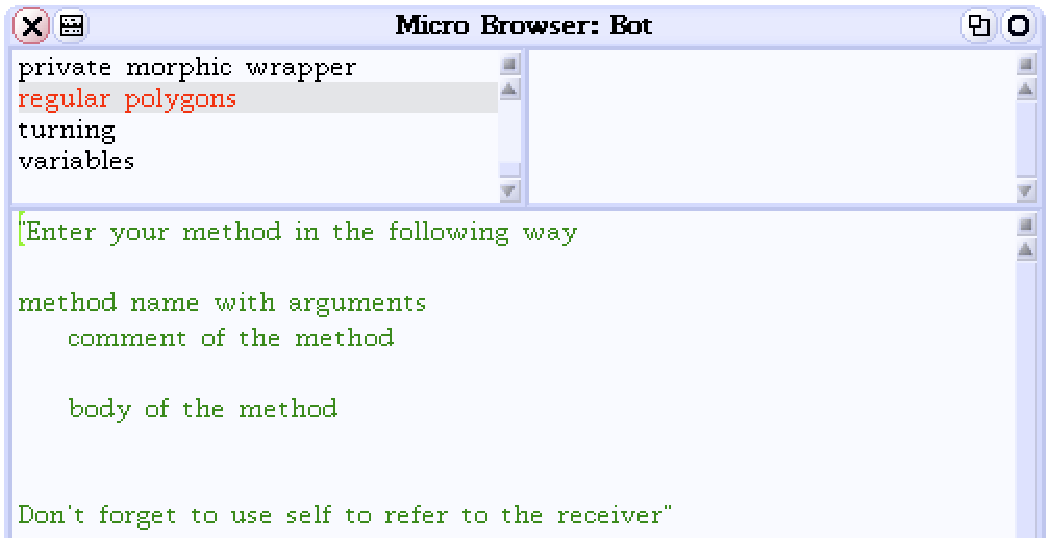
\includegraphics[width=8cm]{tbFour}}
\caption{The new category is ready.\label{fig:categorycreated}}
\end{figure}


\subsection{Defining your First Method}\label{sec:definingmethod}
If the category to which you want to add your method is not selected,
select it. Then type the contents of \methodref{mth:square}
(shown below) into the code editor pane. To do that, select 
all the text in the code editor and start typing your method. 

\begin{method}\label{mth:square}
\textbf{square}
   "Draw a square 100 pixels wide"
   
   4 timesRepeat: 
                [ self go: 100.
                self turnLeft: 90 ]
\end{method}

Defining a method is a three step process:



\paragraph{1. Typing the method.} Typing code into the code editor 
pane works exactly as with the script editor. First delete the reminder text that is in the code editor pane. To make this quick, just point your mouse at 
the beginning of the editor pane before the first character and click. This will select all of the code editor text. Once you finish typing the new method, your screen should look like Figure~\ref{fig:firstMethod}.

\begin{figure}[h]
\centerline{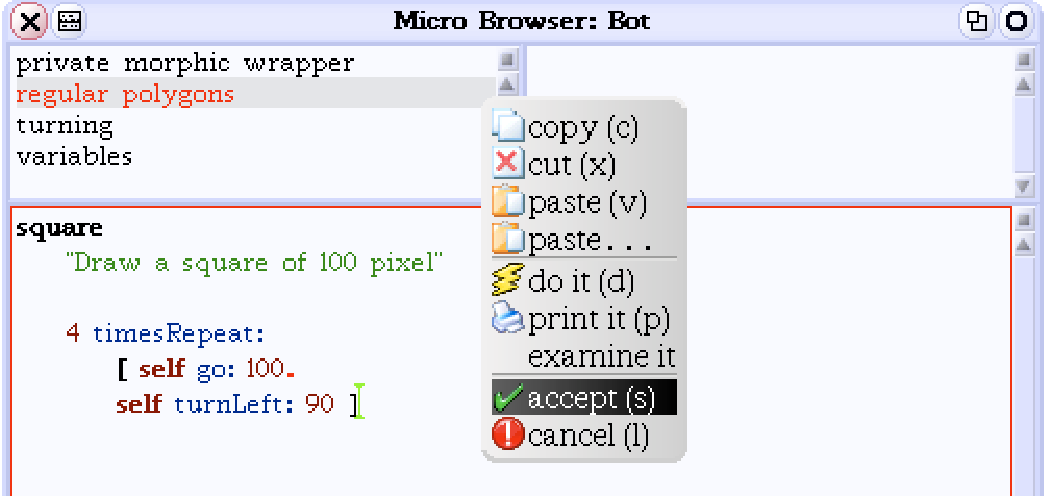
\includegraphics[width=10cm]{tbFive}} 
\caption{You have typed in the method \ct{square}. Now you should compile it using the code editor menu.\label{fig:firstMethod}}
\end{figure}

\paragraph{2. Compiling the method.} As shown by Figure~\ref{fig:firstMethod}, click to bring up the menu  for the code editor and select the option \menu{Accept}.
This compiles the method \ie transforms its definition into a representation that the computer can understand and execute. A new method named \ct{square} appears in the method list.  If you made a mistake while typing the method, \sq will report the error as it would for a script.

If you define  the method correctly, you should be able to compile it without \sq reporting any errors. The browser will then reflect the fact that the compilation is done and that robots can now understand messages with the new method, by showing the new method's name in the method list (see Figure~\ref{fig:methodskeleton}).

%	\begin{figure}
%	\centerline{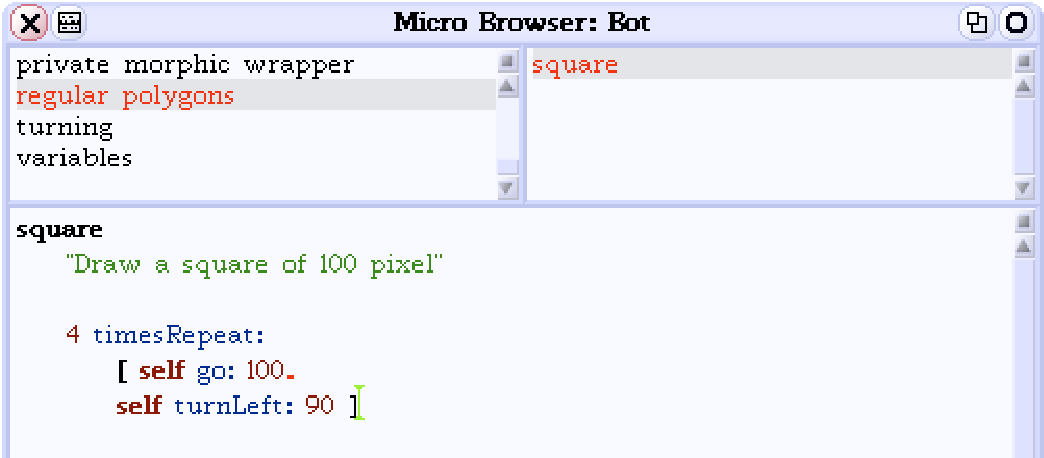
\includegraphics[width=15cm]{tbSix}} 
%	\caption{You have typed \newcommand{\remove}[1]{the method} and \newcommand{\replace}[2]{compile}{compiled} the method \ct{square} 
%	\newcommand{\replace}[2]{now the}{. The} browser reflects the fact that \newcommand{\replace}[2]{robot}{robots} can understand messages with the 
%	new method.\label{fig:compileMethod}}
%	\end{figure}


\paragraph{3. Testing the method!} You  have not finished yet, because 
the method you defined could be wrong. You should test it.  Execute the
\scriptref{src:againSquareMethod}. You should get one black and one red square.

Notice that a method can be reused several times, as demonstrated by \scriptref{src:againSquareMethod}.  This is old news. You have used this fact since the beginning of this book: messages such as \go, \turnLeft and so on, are methods defined in the same way as the method \ct{square}. 

%%%%%%%%%%%%%%%%%%%%%%%%%%%%%%%%%%%%%%%%%%%%%%%%%%%
\section{What's in a Method?}
I asked you to type a method without much explanation. Now is the time to
analyze the structure of the method. 

A method is composed of a \emph{name}, an optional \emph{method comment} and a \emph{method body} (a sequence of messages) as shown by Figure~\ref{fig:methodskeleton}. The method name can also contain parameters (see
chapter~\ref{ch:argumenting}), and the method body can also
define local variables using vertical bars \ct{|} and \ct{|}.

\begin{figure}[h]
\centerline{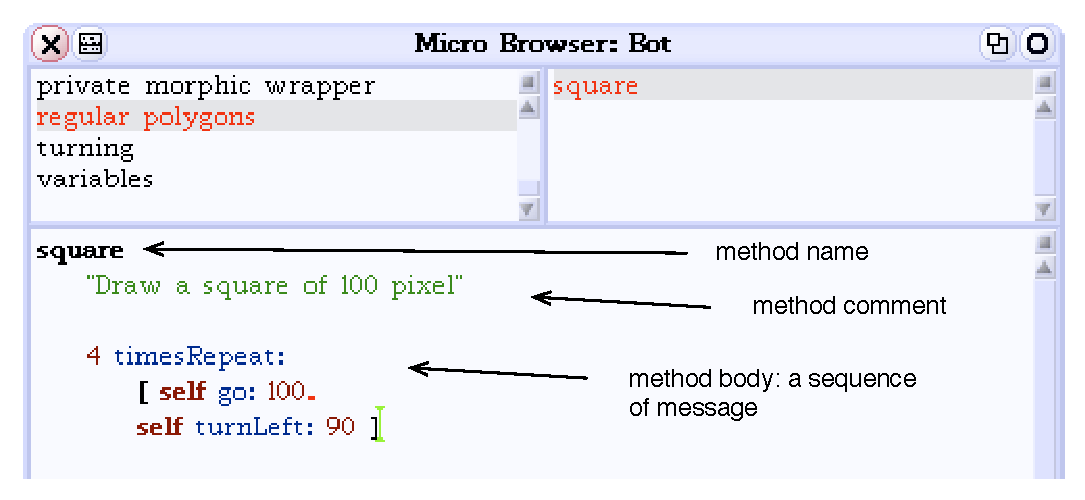
\includegraphics[width=15cm]{tbSixAnnotated}} 
\caption{A method is composed of a name, a method comment and a 
method body. \label{fig:methodskeleton}}
\end{figure}

\largecadre{A method name should always represent what the method does, not how it does it.}

\begin{description}

\item[Method Name.] 
A method name should always represent what the method does, not how it does it.  When you want somebody to open a door, 
you don't explain all the physics and mathematics involved. It is the 
same for methods. 

Method names without parameters such as 
\ct{square} follow the same syntax as variable names. They are 
composed of alphanumeric characters (letters and digits), and start with a
lowercase character. In our case the method name is \ct{square}.

\item[Method Comment.]
A comment consists of text enclosed between double quotes
(\ct{"}). The text cannot contain any double quotes. However a
comment can be as long as you like, and can continue
over several lines. 


In general a comment explains the purpose and the effect of the method. It explains how the method can be used, not how the method does its job. Anyone who wants to know how the method works can read the method's body.


If the method name is clear enough, the comment may be omitted.  
In our case the method comment is:
\begin{nalltt}
   "Draw a square 100 pixels wide"
\end{nalltt}

\item[Method Body.] After the comment comes the method definition itself
\ie the sequence of messages that are executed in response to a message. In our case the 
method body is: 
\


\begin{nalltt}
   4 timesRepeat: 
         [ self go: 100.
         self turnLeft: 90 ]
\end{nalltt}
\end{description}
       
\largecadre{A method is a named sequence of messages. It is composed of
a name, a comment and a sequence of messages. Once a method for robot is defined, any robot can execute it in  response to a message with the same name.}       

\subsection{Script vs. Method: an Analysis}
Let's compare  \methodref{mth:square2} with \scriptref{src:againSquare2}. You can see these differences: (1) The line declaring the variable \caro is not in the method; (2) the line creating the robot is not there, either and (3) in the rest of the method, the variable \caro is replaced by \self.


\noindent
\begin{minipage}{7cm}
\begin{scriptwithtitle}{A simple square}\label{src:againSquare2}
\textbf{| \caro |
\caro := \Turtle new.}
4 timesRepeat: 
         [ \caro turnLeft: 90.
         \caro go: 100 ]
\end{scriptwithtitle}\end{minipage}
\hfill
\begin{minipage}{7cm}
\begin{method}\label{mth:square2}
\textbf{square}
   "Draw a square 100 pixels wide"
   
   4 timesRepeat: 
                [ \textbf{self} go: 100.
                \textbf{self} turnLeft: 90 ]
\end{method}
\end{minipage}


Remember that a robot method represents a sequence of messages which can be sent to \emph{any} robot: the robot referred to by the variable \caro is not necessarily the
receiver of the message \ct{square}. \daly could also be the receiver of the message \ct{square} as we saw in \scriptref{src:againSquare2}. 

Also, the message \ct{square} is sent to an \emph{existing}
robot. There is no need to create a robot since the one we want to send message to already exists. This implies that while defining the method \ct{square}, you need a way to refer to the object that will receive the message \ct{square}. 

In fact, we want to send the sequence of messages specified within the method body to the specific object receiving the message \ct{square} and to no other. Therefore we need a way to refer to the receiver of a message.  This is the purpose of \self. Inside a method, \self represents the object receiving the  message.


\paragraph{The \self variable.}
If you remember the discussion of Chapter~\ref{ch:variables}, a variable is just a named placeholder for an object. In particular, I emphasized  that the same variable could be used to point to different objects at different times.

In the case of a method, the variable \self points to the object that received the message: when the message \ct{\caro\ square} is executed \self refers to the robot named \caro, and when the message \ct{\daly\ square} is executed \self refers to the robot named \daly. 

\largecadre{Inside a method the variable \ct{self} represents the 
object that received the message.\\ \\
For example: when the message \ct{\caro\ square} is executed \self refers to the robot named \caro, and when the message \ct{\daly\ square} is executed \self refers to the robot named \daly.}

\self is a special variable because you cannot change its value. Only \sq can assign the value of \self. That's why \self does not have to be declared between vertical bars \ct{|}. Moreover, \self can only the used inside a method definition.


\largecadre{
When the method code needs to send a message to the receiver, send the message to \self.  \\ \\
For example, in the method \ct{square} one need to turn the robot, so the message \ct{turn: 90} is sent to \self, that is the robot that will receive the message \ct{square}. 
}

\paragraph{Method or Not: That's the Question.} At this stage you may be tempted to go back and convert all the scripts you have written into methods. This is not advisable, because not all scripts are worth turning into a method. In general, one should define a method when the sequence of messages is general enough to be used several times.


\section{Returning a Value}
A method can also return a value by using the character up arrow \^\, also called  \index{return} \index{caret} \index{returning a value} a \emph{caret}.

Imagine that you want to have a method that returns the distance that a robot should move in one movement. You can define the method \ct{maxDistance} shown in~\ref{mth:maxLength}. In this example the method is simply returning a numbe, but we could instead return the result of some complex expression. 

\begin{method}\label{mth:maxLength}
\textbf{maxDistance}
   "returns the maximum distance to move"

   ^ 100
\end{method}

By default every method returns the message receiver. The method~\ref{mth:squareEquivalent} is equivalent to the method \ct{square} defined previously. In fact at the end of every method there is an implicit expression \^ \self. However in this book you do not have to worry about that. 

\begin{method}\label{mth:squareEquivalent}
\textbf{squareEquivalent}
   "Draw a square 100 pixels wide"
   
   4 timesRepeat: 
              [ self go: 100.
              self turnLeft: 90].
   ^ self
\end{method}

In this book, you will not use this feature much, but it is important to know that a method always returns a value. 

\section{Pattern Drawing}\label{sec:newart}
Now it is time to practice. As you have seen, it is quite easy to transform a script into a method.  Many seasoned programmers use scripts to test ideas. When the feasibility of an idea has been proven in the form of a script, they move the code of the script into a method for later reuse. The next exercise trains you to do exactly this.
Let's consider the following script~\ref{src:artNouveau} which draws a geometric shape. 

\begin{scriptfig}{artNouveauScr}{A Simple Pattern}\label{src:artNouveau}
| \caro |
\caro := \Turtle new.
\caro go: 100 ;
        turnLeft: 90 ;
        go: 100 ;
        turnLeft: 90 ;
        go: 50 ;
        turnLeft: 90 ;
        go: 50 ;
        turnLeft: 90 ;
        go: 100 ;
        turnLeft: 90 ;
        go: 25 ;
        turnLeft: 90 ;
        go: 25 ;
        turnLeft: 90 ;
        go: 50
\end{scriptfig}

\begin{exonofig} \label{exo:artNouveau}
Create a method named \ct{pattern} which produces the figure drawn by \scriptref{src:artNouveau}.
\end{exonofig}

You now can use this method in a script to draw a frame.
\begin{scriptfig}{artNouveauFourScr}{A Frame} 
\label{src:artNouveauFrame}
| \caro |
\caro := \Turtle new.
4 timesRepeat: [ \caro pattern ; go: 50 ]
\end{scriptfig}

At this point, some astute reader might ask: why don't we create a
method ---named \ct{frame50}, for example--- corresponding to
that of \scriptref{src:artNouveauFrame}?. This is indeed possible
since \emph{any method created for a robot can be reused
by another robot method}. This is the topic of the next chapter. 

\begin{exonofig} \label{exo:artNouveauFrame50}
Create a method named \ct{frame50} which produces the picture produced by Script \ref{src:artNouveauFrame}. 
\end{exonofig}

\comment{
Let's convert one script, namely \scriptref{src:petal}
\newcommand{\replace}[2]{drawing}{that draws} a petal.
\begin{exonofig} \label{exo:mthPetal45}
Write a method named \ct{petal} corresponding to 
\scriptref{src:petal}. 
\end{exonofig}

In order to test whether the new method you created is correct,
you must write a simple script to test it, a script similar to
Script \ref{src:petal}. After \newcommand{\replace}[2]{this}{that}, try \newcommand{\replace}[2]{to use}{using} the method in a
more complex script.
\begin{exonofig} \label{exo:usePetal45}
Rewrite the script you \newcommand{\remove}[1]{have} made for Exercise \ref{exo:flower} to
use the new method \ct{petal45}.
\end{exonofig}
}

\summa

\begin{enumerate}
\item A method is a named sequence of messages. It is composed of
a name, a comment and a sequence of messages. Once a method is defined, any robot can execute it in response to a message with the same name.

\item A method name should always represent what the method does, not how it does it. 

\item A new method for a robot is created using a class Bot Browser \ie a special 
editor for defining methods. 

\item Inside a method the variable \ct{self} represents the 
object that received the message. 

When the method code needs to send a message to the receiver, send the message to \self.
\end{enumerate}


\subsection*{Glossary}
\begin{itemize}
\item Method categories. A method category is a folder in which methods are sorted. It helps you find methods faster. 
\item Method. A method represents a sequence of messages that an object can execute. A method has a name. It is executed when an object receives a message having the same name. 
\item Browser. A browser is a special tool for viewing and editing methods. 
\item Comment. A comment is a piece of text surrounded by "" that explains the purpose of a method. 
\item \self. \self is a variable predefined by \st that always represents the receiver of the message in a method definition. 
\end{itemize}

\ifx\wholebook\relax\else\end{document}\fi
